\chapter{Wstęp}

\section{Od kodu kreskowego do tagu radiowego}

Wraz z dużym postępem techniki oraz elektroniki w ostatnim dziesięcioleciu\cite{lezar_1}, niemal na każdym kroku\footnote{i tutaj tekst} spotykamy się z systemami automatycznej identyfikacji (ang. Auto ID).  Umożliwiają one szybką , wygodną i bezbłędną identyfikacje produktów, sprzętu, ludzi a nawet zwierząt.  co usprawnia działanie systemów logistycznych. Technologie automatycznej identyfikacji znajdują coraz szersze zastosowanie we współczesnym świecie, głównie w obszarze przemysłu i transportu, przez handel, monitoring  po logistykę. Automatyczną identyfikację rozumiemy jako odczytywanie informacji o produkcie  w czasie rzeczywistym oraz następnie wprowadzenie tych danych do komputera w sposób w pełni zautomatyzowany czyli bez udziału człowieka.  Czytnik zbiera wszelkie możliwe informacje tym samym  zapewniając jednoznaczną, szybka i bezpieczną identyfikację obiektu.

Do najważniejszych systemów automatycznej identyfikacji zaliczamy:
\begin{itemize}\setlength{\itemsep}{0pt}
    \item kody kreskowe (ang. \emph{bar code}),
    \item karty elektroniczne  (ang. \emph{electronic cards}),ścieżki magnetyczne (ang. \emph{magnetic stripe}),
    \item systemy RFID (ang. \emph{Radio Frequency Identyfication}),
    \item systemy automatycznego rozpoznawania pisma ręcznego ICR (ang. \emph{Intelligent Charakter Recognition}) oraz rozpoznawanie znaków (druku)  OCR (ang. \emph{Optical Character Recognition}),
    \item systemy biometryczne:
	\begin{itemize}\setlength{\itemsep}{0pt}
		\item identyfikacja linii papilarnych,
		\item identyfikacja głosu,
		\item identyfikacja siatkówki oka,
		\item rozpoznawanie twarzy
	\end{itemize}
\end{itemize}

Intensywny i dynamiczny rozwój systemów Auto ID miał swój początek w momencie wprowadzenia kodów kreskowych. Najpopularniejszego obecnie sposobu automatycznej identyfikacji obiektów.

Kod kreskowy inaczej określany jako kod paskowy (ang. bar code) jest graficzną formą zapisu znaków, pod postacią ciemnych i jasnych pasków o zróżnicowanej szerokości, według przyjętej symboliki  (przyjętych reguł budowy danego kodu). Skanowanie kodu odbywa się z użyciem czytnika elektronicznego, który emituje cienką wiązkę światła.

Przesuwając się wzdłuż kodu wiązka lasera jest  pochłaniana przez ciemne paski kodu natomiast odbijana przez jasne fragmenty kodu i odbierana przez fotodiodę.

Siła sygnału, który powstaje w czytniku zależy od tego czy światło jest pochłaniane czy odbijane przez paski kodu, natomiast długość trwania sygnału zleży od grubości pasków. W rezultacie otrzymujemy jest ciąg sygnałów elektrycznych o różnej długości i natężeniu. Impulsy elektryczne tłumaczone są przez dekoder czytnika na cyfry, litery lub inne znaki, i przesyłane do komputera. 

Kody kreskowe są powszechnym i tanim sposób etykietowania produktów. Zaletą tego systemu jest powszechna unifikacja sposobu kodowania. Wadami  natomiast mała pojemność pamięci kodów kreskowych oraz częsty problem z odczytem danych (dane trzeba wprowadzać ręcznie). Duży problem w wielu sytuacjach stanowi również niewielka dopuszczalna odległość kodu od czytnika. 

Technologia kodów kreskowych jest obecnie najpowszechniejszą i najtańszą technologią znakowania produktów, jednak osiągnęła już swoje granice możliwości – w pewnych zastosowaniach jest już niewystarczająca.

Coraz większą popularność zyskuje technika radiowej identyfikacji – RFID. System jest bardzo prosty dzięki temu zyskuje na popularności zarówno przy dużych i kosztownych projektach jak również  niewielkich przedsięwzięciach.

\section{Struktura systemu RFID}

RFID (ang. Radio Frequency  Identyfication) to jedna z najszybciej rozwijających  się automatycznych technologii bezprzewodowej  identyfikacji radiowej. Jest to system tani, wszechstronny i niezawodny. Technologia RFID wykorzystuje sygnał radiowy niskiej mocy do bezprzewodowej transmisji danych pomiędzy czytnikiem lub dekoderem  (ang. reader, interrogator), a znacznikiem, inaczej zwanym transponderem lub identyfikatorem (ang. transponder, tag). Dlatego też nie ma konieczności bezpośredniego kontaktu między etykietą, a czytnikiem.

\subsection{Budowa poszczególnych podzespołów systemu}

W skład typowego systemu RFID wchodzą następujące podzespoły:

\begin{itemize}\setlength{\itemsep}{0pt}
	\item znacznik  (etykieta, transponder, identyfikator, tag, chip, metka) –zbudowany z układu elektronicznego lub microchipa z pamięcią, w którym dane są  kodowane i zapisywane w pamięci podręcznej oraz transmitowane za pomocą anteny nadawczo odbiorczej (często napylanej na warstwie izolatora). Cały układ identyfikatora przytwierdzony jest na nośnika np. papieru, plastiku. 

	Znaczniki RFID mogą zawierać zarówno informacje zapisane w formie elektronicznej (pod postacią danych) jak również naniesiony tekst lub kod kreskowy. 

	Identyfikatory możemy sklasyfikować na dwa sposoby . W zależności od sposobu zasilania oraz od konfiguracji w jakiej występują.

	Pod względem zasilania transpondery dzielimy na: pasywne  (ang. passive) (bez wewnętrznego zasilania) do zasilania  wykorzystują energie pola elektromagnetycznego, która wytwarzana jest przez czytnik oraz aktywne (ang. active) (z własnym źródłem zasilania np. baterią) oraz półaktywne lub półpasywne (ang. semi-active, ang. semi-passive) łączą cech zarówno transponderów aktywnych jak i pasywnych . Transpondery te wyposażone są w baterię zapewniającą zasilanie obwodom elektronicznym, natomiast nie posiadają nadajnika. Zasięg odczytu sięga 100 m, w dużym stopniu jednak zależy od czułości odbiornika w czytniku.  

	Znaczniki aktywne osiągają większą moc sygnału transmitowanego z identyfikatora, ponadto transmisja trwa krócej. Stosuje się je przede wszystkim do identyfikacji pojazdów. Najczęściej używane są znaczniki pasywne. Charakteryzują się brakiem własnego zasilania. Energię czerpią z fal radiowych celem odczytu i transmisji danych.  Konfiguracje w jakich może występować pamięć etykiety RFID to: RO (ang. read only) - tylko odczyt – są programowane podczas produkcji i zawierają numer seryjny (mogą zawierać również inne dane , których nie można modyfikować), RW (ang. read write) - odczyt i zapis – dane mogą być wielokrotnie modyfikowane (pamięć może być podzielona na dwie części: część tylko do odczytu i część w której użytkownik może modyfikować zapisane dane) oraz WORM (ang. write once read many) -jednokrotny zapis i wielokrotny odczyt, część danych zapisana jest trwale, a część może być zmieniona przez użytkownika.
	
	\item czytnik  - zbudowany z mikrokomputera, który weryfikuje poprawność otrzymanych informacji, modułu transmisji radiowej czyli nadajnika i odbiornika  odpowiedzialnych za odczyt i zapis danych w identyfikatorze oraz antenę lub cewkę. Niektóre czytniki posiadają dodatkowo interfejs łączący z komputerem PC (pozwalający na transmisję danych pomiędzy czytnikiem a komputerem).
	
	Oprogramowanie czytnika składa się z warstwy komunikacyjnej i użytkowej. Warstwa komunikacyjna odpowiedzialna jest za techniczną stronę transmisji danych, a warstwa użytkowa jest odpowiada za poprawne działanie aplikacji czyli wymianę, gromadzenia i przetwarzanie informacji. W zależności od budowy układu pracuje na komputerze i/lub serwerze.
	
	Im większy czytnik tym większy jego zakres odczytu.
	
	Klasyfikacji czytników można dokonać według dwóch kryteriów. Pierwszy podział oparty jest na kryterium mobilności czytnika: stacjonarne (pracujące w trybie autonomicznym – cały czas sczytuje etykiety znajdujące się w jego zasięgu lub trybie interaktywnym –w tym trybie komunikacja odbywa się za pomocą aplikacji pracującej na serwerze lub aplikacji klienckiej), ruchome, przenośne.

	Drugi podział klasyfikuje czytniki na podstawie typu interfejsu komunikacyjnego:
	
	Szeregowe (porty RS-232 lub RS-485), sieciowe (z interfejsem sieciowym np. Ethernet).
\end{itemize}

Technologia RFID w ostatnim dziesięcioleciu zyskała miano jednego z najbardziej obiecujących i najprężniej rozwijających się systemów identyfikacji na częstotliwości radiowej.  System RFID pozwala na dużą automatyzację pracy zarówno podczas zapisu jak i odczytu danych. W przeciwieństwie do kodów kreskowych technologia ta nie wymaga bezpośredniej widoczności pomiędzy etykietą, a czytnikiem oraz daje możliwość czytania i przetwarzania wielu etykiet równocześnie.

\section{Organizacja systemu RFID}

Zasada działania systemu opiera się na systemie komputerowym z bazą danych (w którym przechowywane  są wszystkie dane o ,,zametkowanym” produkcie)  oraz dwóch modułach identyfikacji radiowej: identyfikatorze i czytniku. Identyfikator – mały układ scalony z umieszczoną wewnątrz anteną w zależności od potrzeb i przeznaczenia zatopiony w plastiku, żywicy lub w formie etykiety samoprzylepnej na opakowaniu czy urządzeniu Każda etykieta posiada swój indywidualny niepowtarzalny numer identyfikacyjny ID, który odnosi się do konkretnej bazy danych. W celu odczytania danych z tagu, nadajnik czytnika RFID emituje pole elektromagnetyczne o częstotliwości rezonansowej układu odbiorczego. Antena dipolowa transpondera na  swoich końcach w skutek wywołanej różnicy  potencjałów indukuje prąd i magazynuje energię w kondensatorze.  Zgromadzona energia pobudza identyfikator do wysyłania odpowiedzi zawierającej kod znacznika. 

Czytnik wyposażony w antenę odbiorcza o dużej czułości, wykrywa, filtruje, demoduluję i dekoduje odebrane fale, tak aby odczytać odpowiedzi z transponderów.

Istnieje możliwość czytania i przetwarzania wielu etykiet (znajdujących się w zasięgu czytnika) równocześnie. Dane zapisane na etykiecie można odczytać w dowolnym momencie. 

Znaczniki, które nie  mają własnego zasilania (znaczniki pasywne), zasilane poprzez pole elekromagnetyczne magazynują energię w kondensatorze, która następnie zasila poszczególne obwody transpondera. Stosunkowo małe wymiary i niski koszt  produkcji transponderów pasywnych pozwala na masowe zastosowanie w wielu sektorach gospodarki. Natomiast transpondery aktywne, znajdując się w polu działania czytnika, pobierają energię ze swojej baterii, aby wysłać przechowywane dane, a co za tym idzie zapewniają większy zasięg nawet do kilkuset metrów, jednak są większe i znacznie droższe niż znaczniki pasywne.

\section{Zakresy częstotliwości }

Systemy RFID są jednym z wielu systemów radiowych, dlatego aby zapewnić bezkolizyjność pracy i zniwelować zakłócenia pomiędzy poszczególnymi systemami wprowadzono podział na zakresy częstotliwości.  Dozwolone dla systemów RFID przedziały częstotliwości zawarte są w pasmie radiowym ustandaryzowanym na całym świecie pod nazwą ISM (ang. Industrial, Scientific, Miedical). Jest to pasmo nielicencjonowane w zamyśle przeznaczone do zastosowań przemysłowych, badawczych i medycznych. Po za pasmem ISM dostępne są dodatkowo niskie częstotliwości poniżej 135 kHZ. Wyróżnić można kilka najpopularniejszych zakresów częstotliwości wykorzystywanych przez identyfikatory RFID:

\begin{itemize}\setlength{\itemsep}{0pt}
	\item pasmo niskich częstotliwości (ang.  LF – Low Frequency) – systemy RFID działają zazwyczaj na częstotliwościach: 125 kHz i 134.2 kHz.
Transpondery LF to zazwyczaj tagi pasywne, które odróżnią się od  transponderów pozostałych pasm częstotliwości małą wrażliwością na występowanie w pobliżu elementów metalowych, substancji płynnych oraz innych elementów wykonanych z dobrych przewodników. Dlatego świetnie sprawdzają się jako identyfikatory narzędzi, podzespołów maszyn, pojazdów czy metalowych kontenerów. Znalazły również zastosowanie w dziedzinie rolnictwa do znakowania zwierząt, leków oraz produktów spożywczych, gdyż pole niskich częstotliwości przenika przez tkanki ciała i płyny.
Wygląd i budowa transpondera LF zależy ściśle od jego przeznaczenia. Transpondery używane jako immobilizery (czyli elektroniczne zabezpieczenia przed niepowołanym uruchomieniem pojazdu) zazwyczaj wbudowane są w kluczyk natomiast cewka anteny czytnika RFID umieszczona współosiowo w stacyjce samochodu.
   
	\begin{figure}[h!]
	\centering
	    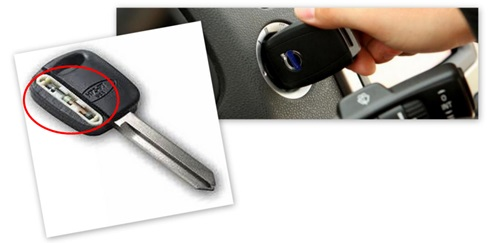
\includegraphics[width=9.32cm]{immobilizer.jpg}
	    \caption{Immobilizer}
	\end{figure}

	Zakres fal do 135 kHz znalazł również zastosowanie zarówno w systemach automatycznej identyfikacji jak i w znakowaniu zwierząt  zarówno hodowlanych jak i domowych.

	\begin{figure}[h!]
	\centering
	    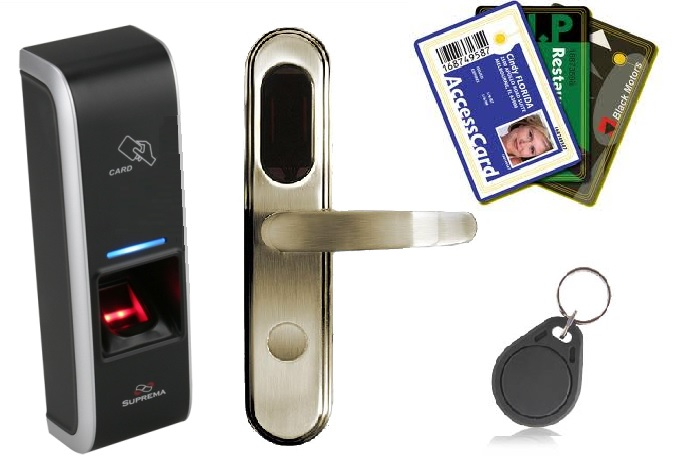
\includegraphics[width=7.27cm]{automatyczna_identyfikacja.jpg}
	    \caption{System automatycznej identyfikacji}
	\end{figure}
	
	\begin{figure}[h!]
	\centering
	    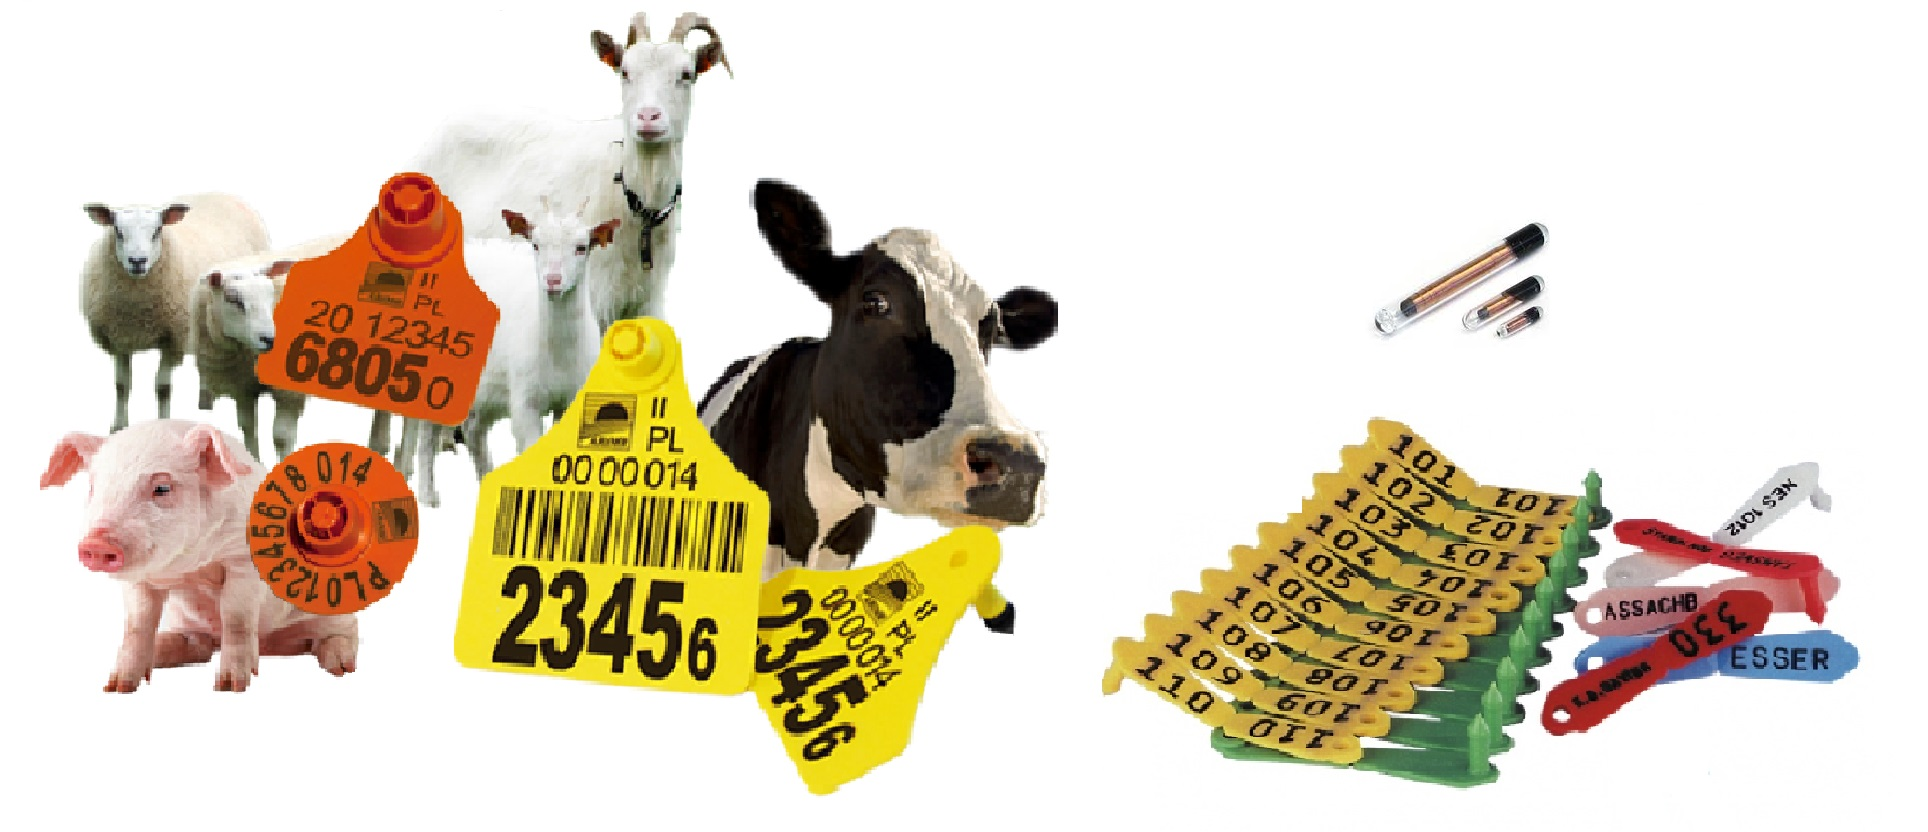
\includegraphics[width=14.34cm]{znakowanie_zwierzat.jpg}
	    \caption{Mikroczipy i kolczyki stosowane do znakowania zwierząt oraz kapsułki (biochipy) do wszczepiania pod skórę}
	\end{figure}
	
	Znaczniki pracujące w paśmie nie należącym do ISM zbudowane są z ferrytowego rdzenia, na którym nawinięte są zwoje (około 100 zwojów) lub w postaci nadrukowanych zwojów na powierzchni materiału. Występują w formie plastikowych kart, krążków, biochipów, pastylek. Wadami tagów RFID pracujących na częstotliwości LH jest: mała szybkość transmisji danych (1-2 kb/sek) - co znacznie ogranicza możliwą do zapisania odczytania ilość danych, niewielki zasięg – około 0.5 metra, podatność na zakłócenia przez urządzenia elektryczne  - co ogranicza zastosowanie w przemyśle. Problemem może być również limit jednoczesnego odczytu nie więcej niż 20 transponderów – ogranicza to pojemność systemu i maksymalną liczbę odczytów jaką może obsłużyć jeden czytnik. 

	\item pasmo wysokich częstotliwości (ang. HF – High Frequency) – najczęściej wykorzystywane częstotliwości w tym pasmie to 6.78 MHz, 13.56 MHz, 27.125 MHz oraz 40.68 MHz. 
Transpondery HF pracujące w zakresie 13.553 MHz – 13.657 MHz (pasmo ISM) to zazwyczaj tagi pasywne. Identyfikatory pracujące na wysokich częstotliwościach wykazują większa wrażliwość na obecność w swoim otoczeniu metali i mniejszy wpływ na zakłócenia elektromagnetyczne pochodzące od  innych urządzeń niż tagi LF. Pamięć tagów HF  ma znacząco większa pojemność, a szybkość komunikacji sięga 20 kbit/s. Główną różnicą w procesie produkcji tagów HF jest zastosowanie anten mniejszych rozmiarów. Antena transpondera HF zbudowana jest zazwyczaj z 3-8 zwojów, nadrukowana jest za pomocą przewodzącego lakieru na podłoże i zaprasowana w etykiecie. Znaczniki możemy spotkać pod postacią samoprzylepnych etykiet (ang. smart label), które programowane są w momencie drukowania etykiety. Zaletami transponderów HF są: znacząco mniejsze koszty wykonania w porównaniu z identyfikatorami LH, co umożliwia ich zastosowanie na większą skalę, niewielka grubość identyfikatora nawet 0,1 mm, możliwy odczyt do 50 znaczników jednocześnie (dzięki wprowadzeniu mechanizmów antykolizyjnych) co pozwala zastosować je do automatycznej identyfikacji produktów i obiektów.  Warunkiem poprawnego odczytu wielu tagów jest zachowanie pomiędzy nimi, odległości co najmniej 2-3 centymetrów. 
\end{itemize}
